\documentclass[a4paper,11pt]{book} 
\usepackage[utf8]{inputenc}
\usepackage[english,frenchb]{babel}
\usepackage[T1]{fontenc} % césure
\usepackage{lmodern} % polices
\usepackage[margin=28mm,bindingoffset=10mm]{geometry} % marges larges : indispensable pour la lisibilité.

\usepackage{pdfpages} % inclure un PDF (article...)
\usepackage{amsmath, mathtools} % maths
%\usepackage{icomma} util. virgule comme séparateur décimal

\pagestyle{headings} %% Personalisation des entêtes standard
\usepackage{slantsc}

\numberwithin{equation}{section}
\numberwithin{figure}{chapter}
\numberwithin{table}{chapter}

\usepackage{titlesec} % passe les gros titres en sansserif
\titleformat{\chapter}[display]{\Huge\sffamily\bfseries}{\chaptername~\thechapter}{1ex}{}
\titleformat{\section}[hang]{\Large\sffamily\bfseries}{\rlap{\thesection}}{2em}{}
\titleformat{\subsection}[hang]{\large\sffamily\bfseries}{\rlap{\thesubsection}}{3em}{}



\begin{document}


{\large

\vspace*{1cm}

\begin{center}

\thispagestyle{empty}

{\bf TH\`ESE DE DOCTORAT DE \\ l'UNIVERSIT\'E PIERRE ET MARIE CURIE}

\vspace*{0.5cm}

Spécialité \\ [2ex] 
{\bf Épidémiologie}\ \\ 

\vspace*{0.5cm}

Ecole doctorale 393 

Épidémiologie et Sciences de l'Information Biomédicale

\vspace*{1cm}


Pr\'esent\'ee par \ \\


\vspace*{0.5cm}


{\Large {\bf Julien RIOU}}

\vspace*{1cm}
Pour obtenir le grade de \ \\[1ex]
{\bf DOCTEUR de l'UNIVERSIT\'E PIERRE ET MARIE CURIE} \ \\

\vspace*{1cm}

\end{center}

\flushleft{Sujet de la thèse :\ \\
\ \\
{\Large {\bf  Analyse quantitative et prédictabilité des épidémies de maladies transmises par les moustiques du genre \textit{Aedes} aux Antilles françaises\\ }}
  

\vspace*{1.5cm} 
\flushleft{soutenue le }\\[2ex]
\flushleft{devant le jury composé de :  }\\[1ex]
\flushleft{\begin{tabular}{r@{\ }ll}
  & M. Pierre-Yves {\sc Boëlle} & Directeur de thèse\\
  & M. Prénom {\sc Nom} & Rapporteur \\
  & M. Prénom {\sc Nom} & Rapporteur  \\
  & M. Prénom {\sc Nom} & Examinateur  \\
  & M. Prénom {\sc Nom} & Examinateur  \\
\end{tabular}}

}


\frontmatter %numbering \roman

\chapter*{Introduction}
% some intro text
\mainmatter % numbering \arabic + reset \page counter
\chapter[Comparer]{Analyse comparative de la transmission du Chikungunya et du Zika} % some content

\section{Introduction}

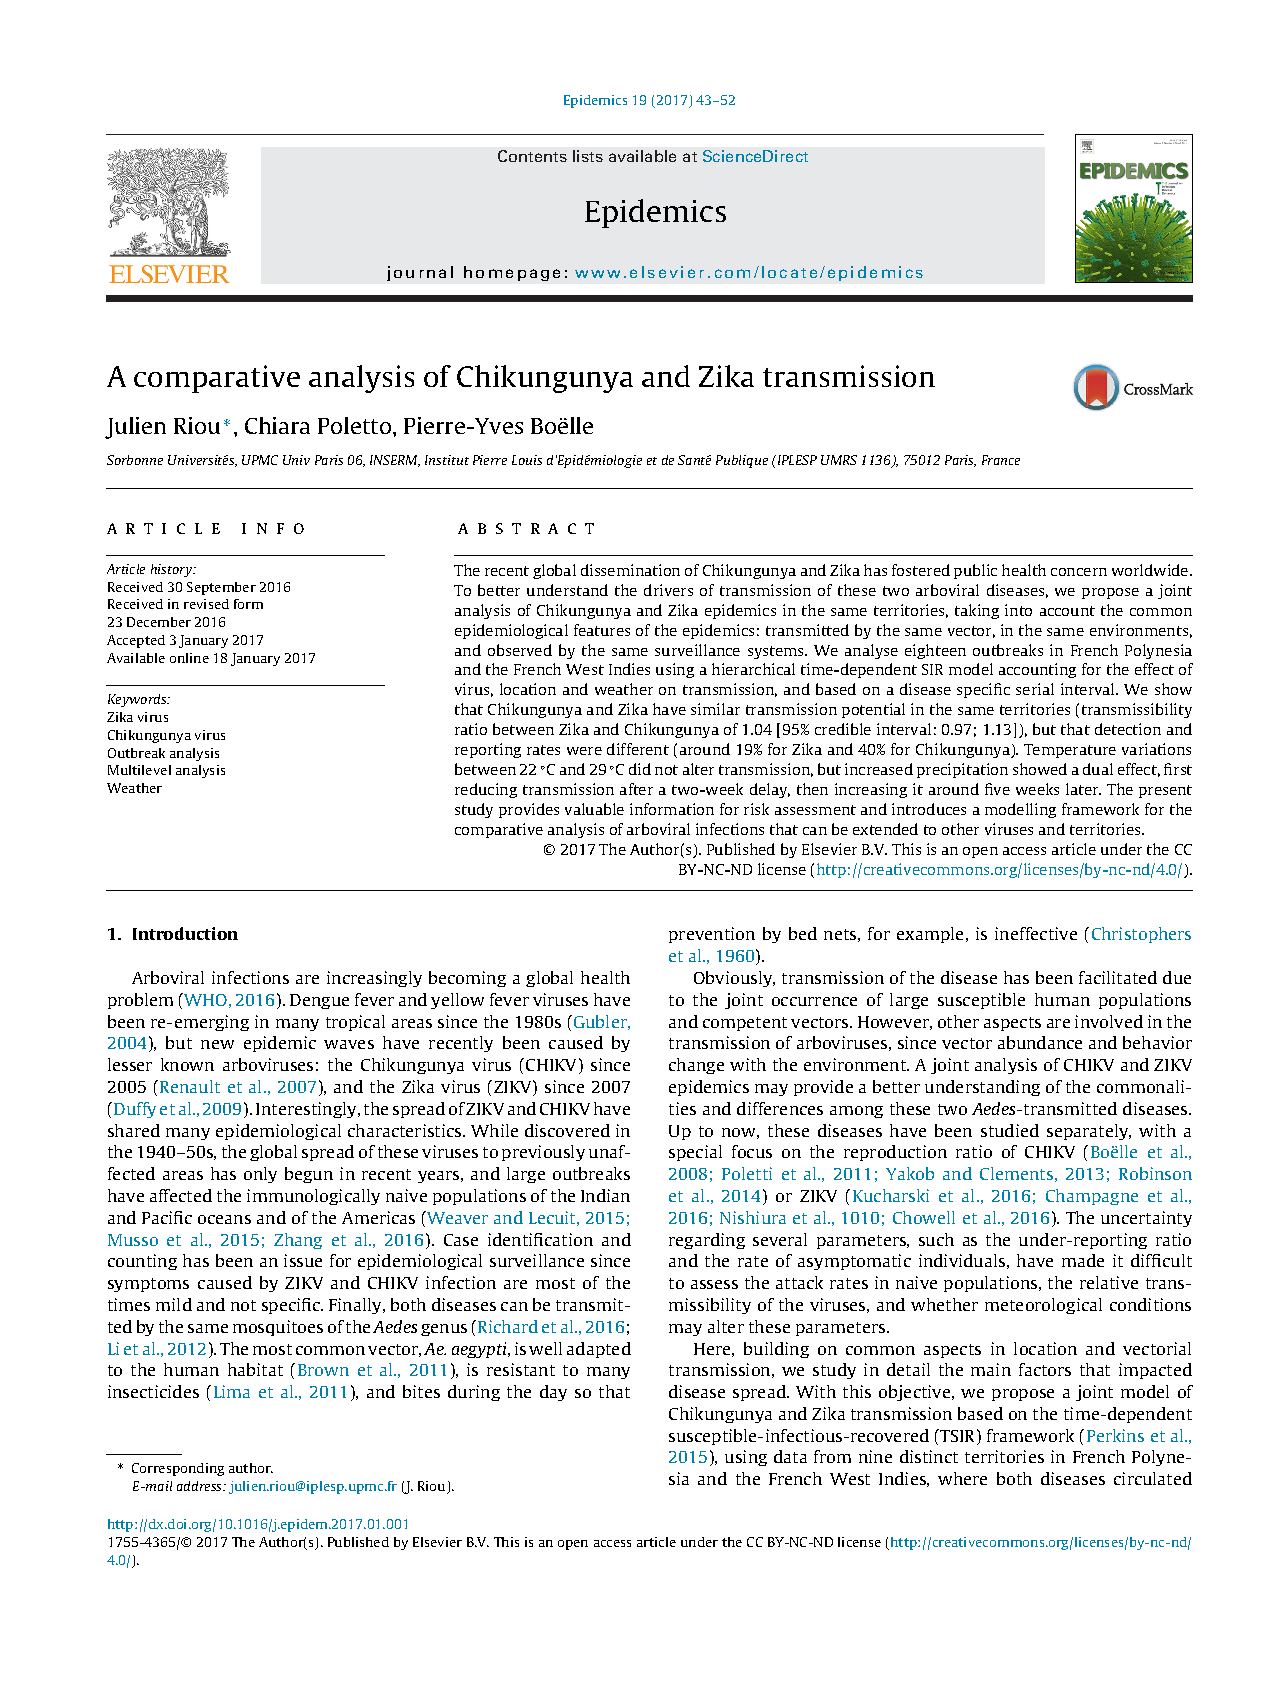
\includepdf[pages={1-10}]{Articles/epidemics.pdf}


\chapter[Prédire]{Utilisation de données historiques pour prédire} % some content



\appendix

\chapter{Annexe A}
\backmatter
% bibliography
\end{document}